\subsection{Impresoras 3D}
	\par
		Es necesario definir el concepto de prototipo porque es el punto de partida para el desarrollo de la tecnología de Prototipado Rapido y consecuentemente, para las impresoras tridimensionales. Podemos definir como prototipo al primer ejemplar que se fabrica de una figura, un invento o elemento físico, y sirve de modelo para fabricar otros iguales.  
	
	\par \noindent
		Los prototipos tiene el propósito de probar suposiciones formuladas en busca de una solución a un problema determinado. Ademas se convierten en un diseño enfocado al usuario, donde es necesario un proceso interactivo entre el propio diseñador y el consumidor. Así mismo, todos los prototipos son objetos de desarrollo de bajo costo, pero en mcuhas ocasiones la necesidad de elaborar varios prototipos o de realizar un prototipo con una estética cuidada, eleva los costes de producción. Por lo tanto, el alto coste de producción de prototipos y tiempo de ejecución de los mismos puede suponer un problema.
	
	\par \noindent
		Los sistemas de Prototipado Rápido surgen con la necesidad de solventar estos problemas en el uso de prototipos, se busca por lo tanto, una manera de elaborarlos con un aspecto cuidado y atractivo para el usuario, con un método de fabricación rápido y fácil de modificar, económicos y que pueden ser probados por el consumidor. Por consiguiente, esta herramienta resultará útil y funcional. Rápidamente estos sistemas de construcción aditiva partirán del desarrollo tecnológico de maquinara destinada a uso industrial. 
				
	\begin{figure}[h]
		\centering
		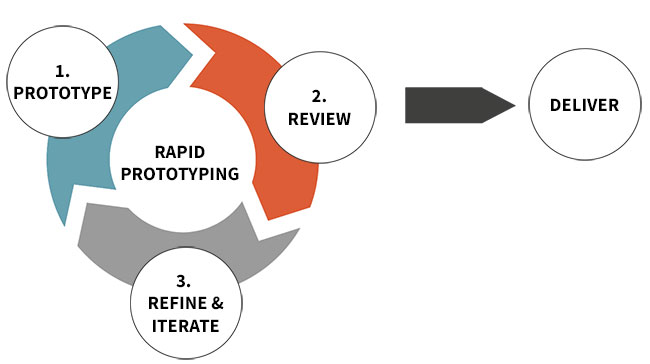
\includegraphics[width=0.7\textwidth]{figura6_rapidproto.jpg}
		\caption{Ciclo del Prototipado Rápido}
	\end{figure}

	\par \noindent
		El Prototipado Rápido se convierte así, en un proceso utilizado para la fabricación de prototipos, los cuales, como hemos visto, son objetos que no estan diseñados a uso final, sino más bien a modo de prueba de diseño.
		
	\newpage
	\thispagestyle{plain}

	\par \noindent
		La impresión 3D, también conocida como impresión tridimensional, es un método para
		producir objetos tridimensionales con un aparato tecnológico al colocar varias capas
		bidimensionales de cierto material una sobre la otra. El proceso es similar a la impresión
		bidimensional en la cual se coloca tinta sobre papel, sin embargo, en la impresión
		tridimensional se coloca plástico sobre una superficie que nos permite fabricar objetos de tres
		dimensiones. Esta tecnología se utiliza principalmente en la producción de prototipos durante
		el diseño de algún nuevo producto.

	\par \noindent
		Durante los últimos años, la tecnología de impresión tridimensional ha avanzado de
		manera exponencial. Este tipo de impresoras se han vuelto cada vez más accesibles y por ello
		ahora es común encontrarlas en fábricas, industrias, instituciones educativas, instituciones de
		investigación e inclusive para uso personal.

	\subsubsection{Técnicas}
	
	\begin{itemize}
		\item SLA (Estereografía): Se basa en las propiedades de una resina fotosensible que se solidifica mediante la proyección de un láser (UV) de frecuencia y potencia concreta.
		
		\begin{figure}[h]
			\centering
			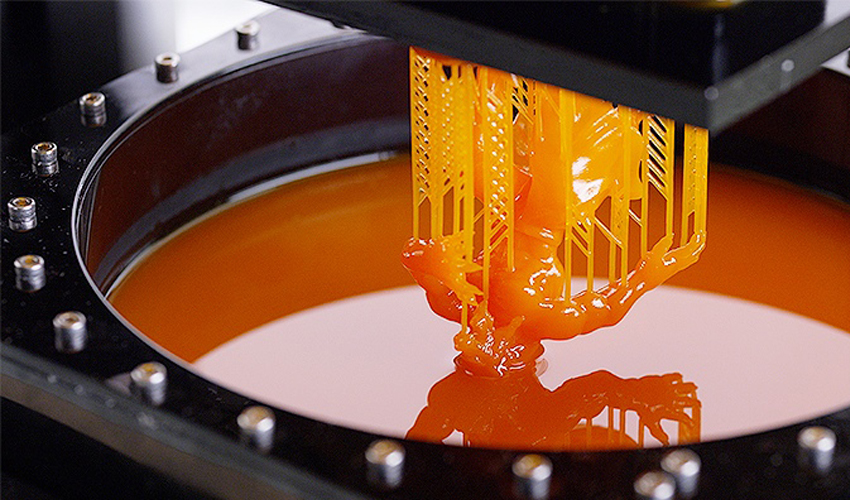
\includegraphics[width=8cm, height=6cm]{figure7_slaprint.jpg}
			\caption{Resultado de impresión tridimensional SLA}
		\end{figure}
	
		\newpage
		\thispagestyle{plain}
			
		\item SLS (Sintetización selectiva laser): En vez de emplear un fotopolímero como ocurre con la SLA, para sintetizarlo, utiliza un compuesto en polvo de diversas clases, normalmente microesferas de poliamida junto con un láser que causa que las partículas se fusionen y solidifiquen. 
		
		\begin{figure}[h]
			\centering
			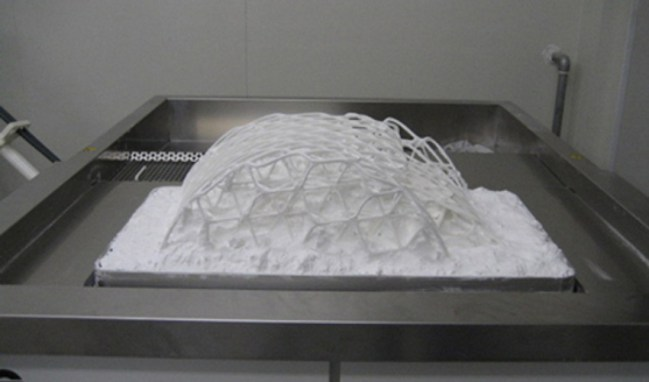
\includegraphics[width=8cm, height=6cm]{figure8_slsprint.jpg}
			\caption{Resultado de impresión tridimensional SLS}
		\end{figure}
		
		\item FDM (Modelado por disposición de hilo fundido): Consiste en la deposición por capas de material normalmente construido por filamentos de polímeros termoplásticos, que se funden y se extruyen por medio de una boquilla, solidificándose cuando salen de dicha boquilla al exterior. Esta técnica es la que utilizaremos en este trabajo.
		
		\begin{figure}[h]
			\centering
			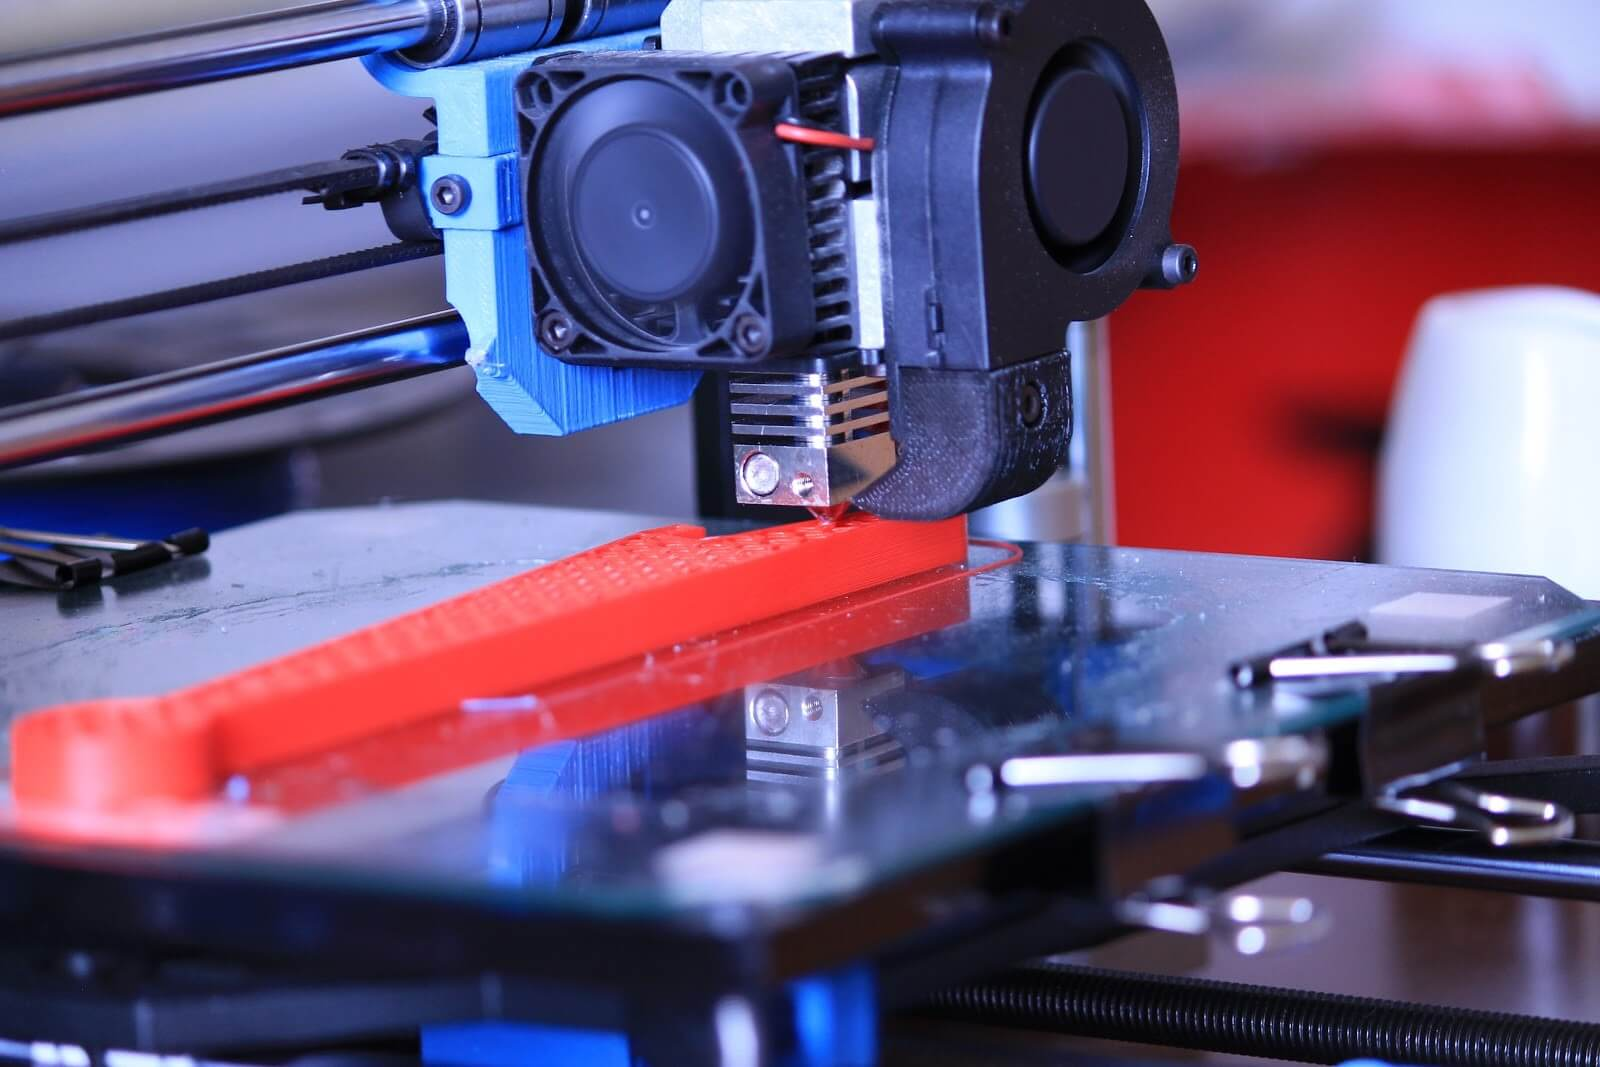
\includegraphics[width=8cm, height=6cm]{figure9_fdmprint.jpg}
			\caption{Resultado de impresión tridimensional FDM y Vista de una boquilla o extrusor}
		\end{figure}
	
		\newpage
		\thispagestyle{plain}
		
		\item SGC (Fotopolimerización): Al igual que en la estereolitografía, la fotopolimerización se basa en la solidificación de
		un fotopolímero o resina fotosensible, sin embargo, en el proceso de
		fotopolimerización se irradia, con una lámpara de UV en vez de con un láser
		ultravioleta. Por lo tanto, necesita una única operación junto con máscaras creadas
		con tinta electroestática en una placa de vidrio.

		\begin{figure}[h]
			\centering
			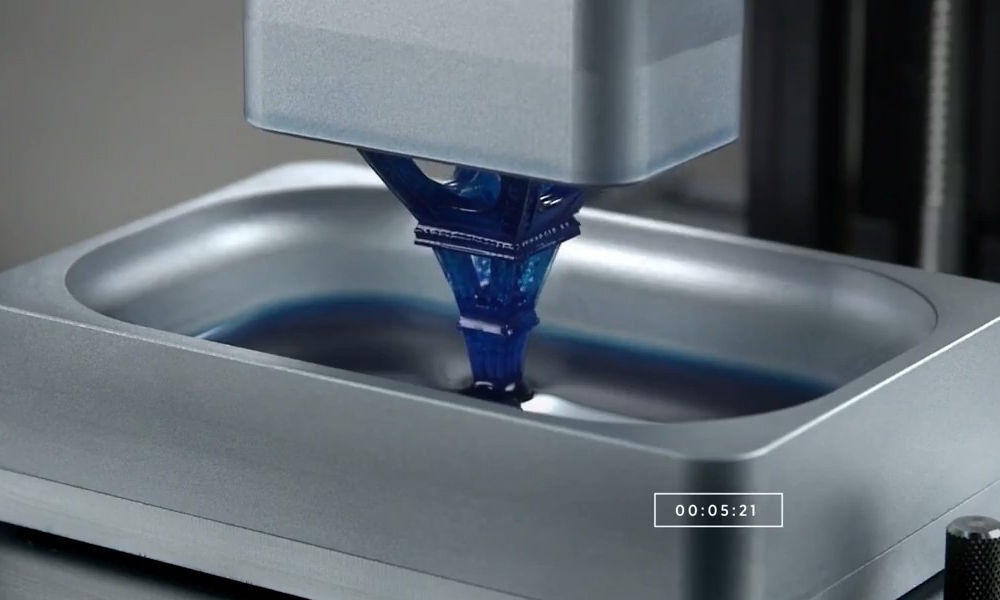
\includegraphics[width=8cm, height=6cm]{figura14_sgcprint.jpg}
			\caption{Resultado de impresora SGC}
		\end{figure}
		
		\item DMLS (Direct Metal Laser Sintering): fue patentado por las empresas ERD y EOS
		(Alemania) en 1994, incluso las primeras investigaciones comenzaron en los años 70. 

		\par \noindent
			La plataforma en la que se realiza la impresión está compuesta de 2 recipientes, cada
			uno activado por un pistón. El primero es recubierto de polvo metálico mientras que el
			segundo se encuentra vacío y situado al nivel de la plataforma. El proceso de
			impresión empieza añadiendo una fina capa de polvo (de una altura máxima
			determinada por el software de la impresora) en el recipiente vacío. El láser de fibra
			fusiona el polvo metálico. Una vez que la materia se consolida, una segunda capa de
			polvo es aplicada con la ayuda del sistema de pistones, y así sucesivamente hasta la
			creación completa de la pieza.
			
		\newpage
		\thispagestyle{plain}
			
		\begin{figure}[h]
			\centering
			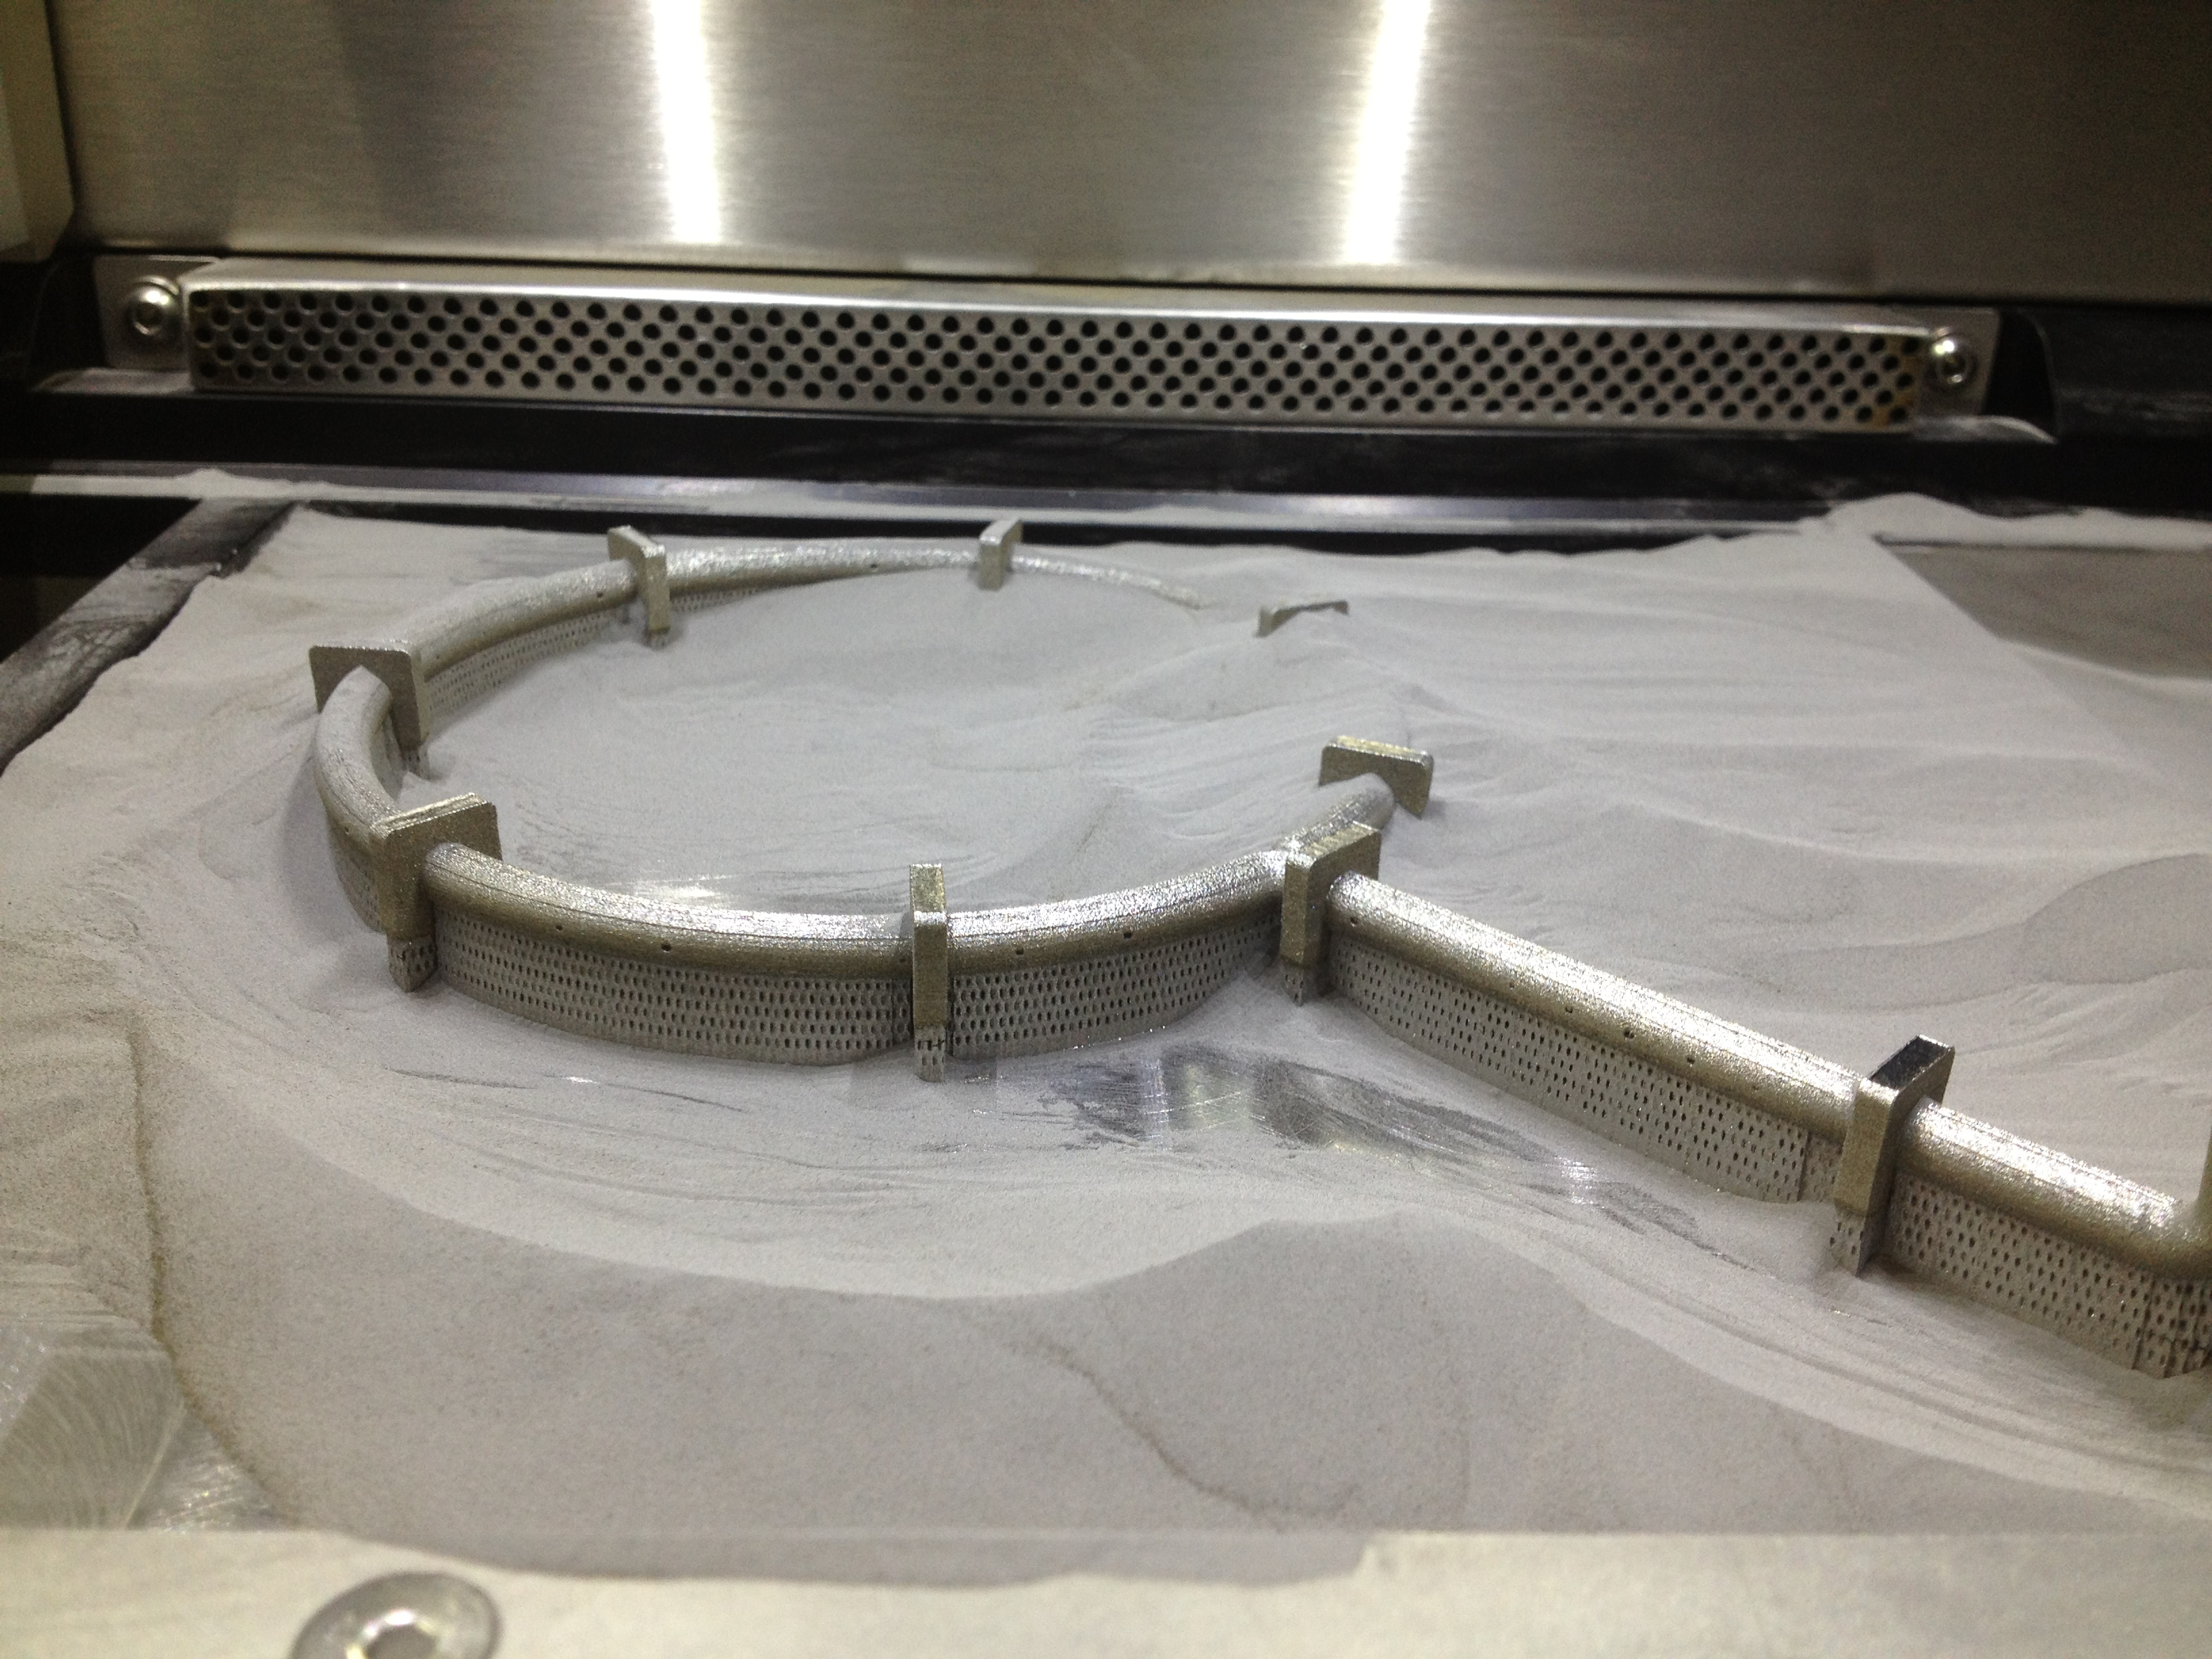
\includegraphics[width=8cm, height=6cm]{figure10_dmlsprint.jpg}
			\caption{Resultado de impresión tridimensional DMLS}
		\end{figure}
			
		\item CLG (Cerámica láser gelificante): La materia prima que se utiliza en la cerámica láser gelificante, es un polvo cerámico
		con un compuesto inorgánico soluble en agua que forma una pasta cerámica. Este
		compuesto es expuesto a un láser de 4W que evapora el agua en una zona
		determinada de la capa, la cual se gelifica localmente para formar capa a capa una
		pieza cerámica en crudo. 
		
		\begin{figure}[h]
			\centering
			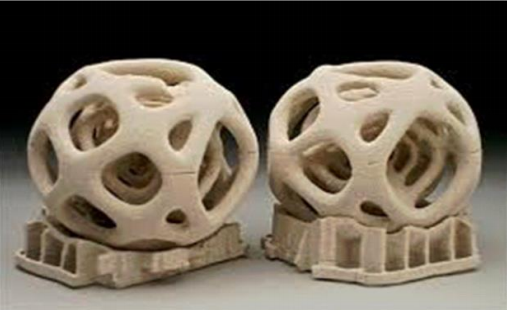
\includegraphics[width=8cm, height=6cm]{figura11_ceramicprint.png}
			\caption{Resultado de impresión tridimensional CLG}
		\end{figure}
		
		\newpage
		\thispagestyle{plain}
		
		\item LOM (Fabricación por Corte Laminado): El proceso consiste en cortar, posicionar y pegar o unir láminas de material como
		papel, arena, cerámica y composites.
		
		\begin{figure}[h]
			\centering
			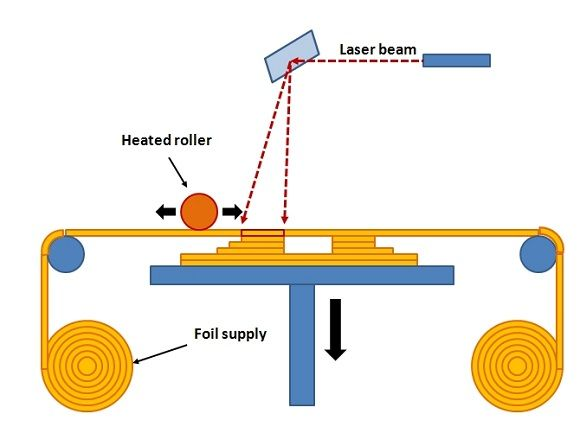
\includegraphics[width=8cm, height=6cm]{figura12_lomprint.jpg}
			\caption{Arquitectura de impresora LOM}
		\end{figure}
		
	\end{itemize}